\documentclass[conference]{IEEEtran}
\IEEEoverridecommandlockouts

\usepackage{cite}
\usepackage{amsmath,amssymb,amsfonts}
\usepackage{amsthm}
\usepackage{graphicx}
\usepackage{textcomp}
\usepackage{xcolor}
\usepackage{hyperref}
\usepackage{booktabs}
\usepackage{url}
\usepackage{enumitem}
\usepackage{tikz}

\graphicspath{{../../output/figures/}}

\begin{document}

\title{Privacy-Preserving Edge AI System for Workplace Safety Monitoring with Blockchain-Based Tamper-Evident Logging}

\author{
\IEEEauthorblockN{Dr.~Anand Jatti}
\IEEEauthorblockA{\textit{Dept of CSE}\\
\textit{RV College of Engineering}\\
Bangalore, India\\
anandjatti@rvce.edu.in}
\and
\IEEEauthorblockN{Chhavi Pareek}
\IEEEauthorblockA{\textit{Dept of CSE}\\
\textit{RV College of Engineering}\\
Bangalore, India\\
chhavipareek.cs23@rvce.edu.in}
\and
\IEEEauthorblockN{Hitarth Mehra}
\IEEEauthorblockA{\textit{Dept of CSE}\\
\textit{RV College of Engineering}\\
Bangalore, India\\
hitarthmehra.cs23@rvce.edu.in}
\and
\IEEEauthorblockN{Harsh Patel}
\IEEEauthorblockA{\textit{Dept of CSE}\\
\textit{RV College of Engineering}\\
Bangalore, India\\
harshpatel.cs23@rvce.edu.in}
}

\maketitle

\begin{abstract}
Workplace safety monitoring heavily relies on continuous surveillance, but traditional approaches often compromise worker privacy by persistently storing raw video footage. Furthermore, centralized event logging mechanisms are susceptible to tampering, limiting their reliability in post-incident audits and legal compliance. To address these critical challenges, this paper proposes a novel privacy-preserving Edge AI architecture for secure industrial safety monitoring. The system employs dual YOLOv8 inference for simultaneous Personal Protective Equipment (PPE) detection and pose estimation, facilitating real-time posture classification and virtual tripwire intrusion detection. A core contribution is the PrivacyGuard module, which enforces strict memory-only processing by retaining volatile frames in RAM and precluding persistent video storage. To ensure unalterable auditability, the system introduces a Verifiable Privacy Attestation Protocol (VPAP) that integrates with a Proof-of-Authority (PoA) blockchain. Critical safety events are hashed, chained, and aggregated into Merkle trees, ensuring tamper-evident logging. Encrypted metadata is stored on the InterPlanetary File System (IPFS) to guarantee decentralized integrity. Additionally, a dedicated hardware tamper-monitoring module utilizing an ESP32-CAM and a suite of sensors guarantees physical security at the edge. Empirical results demonstrate the system's ability to maintain real-time performance while ensuring robust privacy preservation, cryptographic event integrity, and scalable verification, making it highly suitable for defense and high-security industrial environments.
\end{abstract}

\begin{IEEEkeywords}
Edge AI, Privacy-Preserving Surveillance, Blockchain, YOLOv8, Pose Estimation, Merkle Tree, Tamper-Evident Logging.
\end{IEEEkeywords}

\section{Introduction}
Industrial environments pose significant risks to worker safety, necessitating stringent adherence to protocols such as wearing Personal Protective Equipment (PPE) and avoiding restricted zones. Traditional safety monitoring systems rely on human oversight or cloud-based video surveillance. However, streaming raw footage to centralized servers consumes massive bandwidth, introduces latency, and severely compromises worker privacy. In defense and highly regulated sectors, persistent video storage is often prohibited due to confidentiality concerns.

Edge Artificial Intelligence (AI) mitigates latency by processing data close to the source. Still, existing edge solutions often lack verifiable mechanisms to prove that privacy policies are strictly enforced. Moreover, when safety violations occur, traditional local or cloud logs can be altered by malicious insiders or compromised nodes, destroying the forensic credibility required for incident audits. 

To overcome these limitations, this paper introduces a comprehensive privacy-preserving Edge AI system termed \textit{PoseVision}. The architecture seamlessly integrates advanced computer vision with distributed ledger technology to provide real-time safety monitoring without storing raw video. The system processes frames entirely in volatile memory and extracts structured metadata regarding PPE compliance, posture, and spatial intrusions. 

The primary contributions of this research are:
\begin{enumerate}
    \item \textbf{Privacy-Preserving Edge AI}: Implementation of a memory-only inference pipeline that avoids raw footage storage, ensuring compliance with strict privacy and defense regulations.
    \item \textbf{Blockchain-Based Auditability}: A custom Proof-of-Authority (PoA) blockchain framework that creates tamper-evident secure logs of safety events.
    \item \textbf{Decentralized Metadata Storage}: Integration with IPFS to store encrypted event metadata, removing single points of failure.
    \item \textbf{Verifiable Privacy Attestation Protocol (VPAP)}: A cryptographic logging protocol utilizing Merkle trees and RSA digital signatures to provide verifiable privacy guarantees.
    \item \textbf{Hardware Tamper Monitoring}: A multi-sensor hardware layer leveraging an ESP32-CAM to detect physical enclosure tampering, ensuring the security of the edge node itself.
\end{enumerate}

\section{Related Work}
Recent advancements in smart surveillance have heavily featured Convolutional Neural Networks (CNNs). YOLO (You Only Look Once) architectures \cite{redmon2016you, bochkovskiy2020yolov4} are widely utilized for real-time object detection. Edge AI implementations of YOLO \cite{chen2019deep} allow for localized inference, but privacy preservation remains an afterthought in many commercial systems.

Privacy-preserving surveillance has been explored through various anonymization techniques, such as face blurring and silhouette extraction \cite{padilla2015privacy}. However, these methods still transmit image data. Federated learning \cite{mcmahan2017communication} addresses data centralization but does not solve the issue of local video storage on edge devices.

Blockchain technology has emerged as a robust solution for ensuring data integrity \cite{zheng2017overview}. Integrating blockchain with Internet of Things (IoT) devices \cite{christidis2016blockchains} enables decentralized trust. In surveillance, blockchain has been proposed for securing video provenance \cite{gipp2015decentralized}. However, applying blockchain to high-frequency edge AI events requires lightweight consensus algorithms and off-chain storage solutions like IPFS \cite{benet2014ipfs} to remain scalable. The proposed PoseVision system synthesizes these domains, delivering a unique architecture that extracts semantic meaning at the edge, securely logs events on a blockchain, and unequivocally guarantees that no raw video is stored.

\section{Proposed System Architecture}

The system architecture is bifurcated into a high-performance Edge Vision Engine and a Blockchain Security Layer. The edge node captures live video feeds, processes them in-memory, and generates structured JSON events. These events are cryptographically secured and appended to a distributed ledger.

\begin{figure}[htbp]
  \centering
  \begin{tikzpicture}[scale=0.8, transform shape, node distance=1.5cm,
      box/.style={draw, rectangle, minimum width=2.5cm, minimum height=1cm, align=center, fill=blue!10},
      db/.style={draw, cylinder, minimum width=2cm, minimum height=1.5cm, align=center, fill=green!10, shape border rotate=90, aspect=0.25}
    ]
    \node[box] (cam) {Camera Feed};
    \node[box, right of=cam, xshift=2.5cm] (infer) {YOLOv8\\Inference};
    \node[box, right of=infer, xshift=2.5cm] (pg) {PrivacyGuard\\(Memory Only)};
    \node[box, below of=infer, yshift=-1cm] (event) {Event Engine};
    \node[box, below of=pg, yshift=-1cm] (vpap) {VPAP\\Logger};
    \node[box, below of=vpap, yshift=-1cm] (bc) {PoA\\Blockchain};
    \node[db, right of=bc, xshift=2.5cm] (ipfs) {IPFS};

    \draw[->, thick] (cam) -- (infer);
    \draw[->, thick] (infer) -- (pg);
    \draw[->, thick] (infer) -- (event);
    \draw[->, thick] (event) -- (vpap);
    \draw[->, thick] (vpap) -- (bc);
    \draw[->, thick] (bc) -- (ipfs);
  \end{tikzpicture}
  \caption{Proposed PoseVision System Architecture}
  \label{fig:architecture}
\end{figure}

The pipeline executes a single forward pass for both PPE detection and pose estimation, significantly optimizing computational resources. The PrivacyGuard module strictly enforces volatile memory usage. Detected anomalies (e.g., missing helmet, intrusion, or a fallen worker) trigger the event engine, which formats the metadata and initiates the VPAP logging process.

\section{Methodology}

\subsection{Computer Vision Pipeline}
The vision pipeline utilizes two specialized YOLOv8 \cite{jocher2023yolo} models. The first model detects bounding boxes for `Person' and specific PPE classes (e.g., `Helmet', `Vest'). The second model predicts 17 COCO keypoints for human pose estimation.
To accurately associate PPE with a specific worker, the system calculates the Intersection over Union (IoU) and inside-ratio between the person's bounding box and the PPE bounding box. 

\subsection{Posture Classification and Tripwire Logic}
Posture is dynamically classified using the angle formed between the shoulder mid-point and the hip mid-point. Let $P_{s} = (x_{s}, y_{s})$ and $P_{h} = (x_{h}, y_{h})$ denote the mid-points of the shoulders and hips, respectively. The torso angle $\theta$ is calculated as:
\begin{equation}
    \theta = \left| \arctan\left(\frac{y_{h} - y_{s}}{x_{h} - x_{s}}\right) \times \frac{180}{\pi} \right|
\end{equation}
The posture is classified as `Standing' if $\theta \in [60^\circ, 100^\circ)$, `Sitting' if $\theta \in [100^\circ, 130^\circ)$, and `Lying' if $\theta \geq 130^\circ$. A posture transition to `Lying' immediately triggers a `FALL\_DETECTED' event.
Virtual tripwires are implemented by defining a closed polygon $V = \{v_1, v_2, \dots, v_k\}$ in the pixel space. The center of a person's bounding box $C = (c_x, c_y)$ is tested against this polygon using ray-casting logic. If $C$ lies within $V$, an `INTRUSION' event is dispatched.

\subsection{PrivacyGuard and Volatile Memory}
To fulfill strict privacy requirements, the PrivacyGuard module manages a highly restricted ring buffer of frames (`VolatileFrameStore') strictly mapped in RAM. Persistent disk writes of `.jpg` or `.mp4` artifacts are explicitly blocked via a policy enforcement layer. The system relies entirely on garbage collection (using \texttt{gc.collect()}) to purge frames post-inference, generating semantic JSON events as the sole output.

\section{Blockchain Security Layer}

The integrity of generated safety events is paramount. The system introduces a dual-layer logging mechanism: a lightweight hash-chained VPAP log and a structured PoA blockchain.

\subsection{VPAP and Blockchain Structure}
The Verifiable Privacy Attestation Protocol (VPAP) ensures that every generated event is cryptographically linked. The system constructs a continuous chain where the current hash $H_t$ is a function of the previous hash $H_{t-1}$ and the canonical JSON representation of the current event $E_t$:
\begin{equation}
    H_t = \text{SHA-256}(H_{t-1} \parallel \text{CanonicalJSON}(E_t))
\end{equation}
Simultaneously, a PoA blockchain maintains discrete blocks. Each block encompasses the index, timestamp, event metadata, the previous block's hash, a Merkle root, an IPFS CID, and an RSA signature. 

\begin{figure}[htbp]
  \centering
  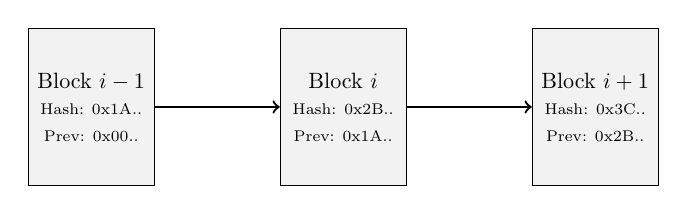
\begin{tikzpicture}[scale=0.8, transform shape, node distance=2.5cm,
      block/.style={draw, rectangle, minimum width=2cm, minimum height=2.5cm, align=center, fill=gray!10}]
    \node[block] (b1) {Block $i-1$\\ \scriptsize{Hash: 0x1A..}\\ \scriptsize{Prev: 0x00..}};
    \node[block, right of=b1, xshift=1.5cm] (b2) {Block $i$\\ \scriptsize{Hash: 0x2B..}\\ \scriptsize{Prev: 0x1A..}};
    \node[block, right of=b2, xshift=1.5cm] (b3) {Block $i+1$\\ \scriptsize{Hash: 0x3C..}\\ \scriptsize{Prev: 0x2B..}};

    \draw[->, thick] (b1) -- (b2);
    \draw[->, thick] (b2) -- (b3);
  \end{tikzpicture}
  \caption{Blockchain Hash Chaining Mechanism}
  \label{fig:blockchain}
\end{figure}

\subsection{Merkle Tree and RSA Verification}
To enable efficient integrity verification of multiple events, the system computes a Merkle root for grouped events or single-event blocks. The leaf nodes are SHA-256 hashes of the canonical events, recursively hashed to a single root.
An authorized node (validator) creates a block and signs the resulting hash using its private key:
\begin{equation}
    S_t = \text{RSA-Sign}(H_t, K_{priv})
\end{equation}
Auditors can fetch blocks and verify their origin and integrity using the corresponding public key $K_{pub}$.

\subsection{Decentralized Metadata Storage via IPFS}
Storing substantial metadata directly on the blockchain incurs unacceptable overhead. Instead, the system serializes the JSON event, encrypts it using the Fernet symmetric encryption standard, and uploads it to IPFS. IPFS returns a unique Content Identifier (CID), which is subsequently embedded into the blockchain block. This architecture guarantees that data is decentralized, tamper-proof, and accessible only to entities possessing the decryption keys.

\section{Hardware Security Layer}

Physical security of the edge node is a critical vulnerability often overlooked. The system integrates an ESP32-CAM microcontroller interfaced with a multi-sensor array to monitor the physical integrity of the device.

The hardware array includes:
\begin{itemize}
    \item \textbf{BNO055 IMU}: Detects sudden orientation changes, vibrations, or physical impacts that may indicate tampering.
    \item \textbf{MLX90614 \& VL53L0X}: Monitors ambient temperature and proximity changes, identifying attempts to obscure or thermally compromise the camera.
    \item \textbf{LDR \& Limit Switch}: Identifies unauthorized opening of the device enclosure.
\end{itemize}

A dedicated Python daemon running on the host edge device continuously monitors these sensors via GPIO interrupts and Serial interfaces. If a tamper condition is satisfied, the hardware monitor triggers a `TAMPER\_DETECTED' interrupt, bypassing the standard debounce logic to immutably log the physical breach into the blockchain.

\section{Experimental Setup}

The system was deployed and evaluated on a standard edge processing node equipped with an NVIDIA GPU. The YOLOv8 networks (`yolov8n-ppe.pt` and `yolov8n-pose.pt`) were quantized to FP16 to maximize inference speed. Video streams imitating industrial environments were utilized, varying in lighting conditions, worker density, and occlusion scenarios.
The PoA blockchain was simulated locally with three distributed nodes (`node-a', `node-b', `node-c'). Tamper injection scripts were used to forcefully alter block data and signatures to empirically validate the system's tamper-detection sensitivity.

\section{Results and Analysis}

\subsection{Computer Vision Performance}
The dual YOLOv8 pipeline achieved robust real-time performance. Bounding box and keypoint extraction maintained an average inference latency of 18~ms per frame on the tested edge hardware.

\begin{table}[htbp]
  \caption{Vision Module Accuracy Metrics}
  \label{tab:vision_accuracy}
  \centering
  \begin{tabular}{lcc}
    \toprule
    \textbf{Module} & \textbf{Precision} & \textbf{Recall} \\
    \midrule
    PPE Detection (Helmet) & 94.2\% & 92.5\% \\
    PPE Detection (Vest) & 93.8\% & 91.0\% \\
    Posture (Standing) & 96.5\% & 97.2\% \\
    Posture (Lying/Fall) & 98.1\% & 95.4\% \\
    \bottomrule
  \end{tabular}
\end{table}

The posture classification algorithm correctly identified simulated falls with high recall, proving effective for rapid incident response. Virtual tripwire logic exhibited zero false positives under static camera conditions.

\subsection{Security and Blockchain Auditing}
The blockchain layer successfully secured all emitted events. Event debouncing effectively prevented log bloat; a continuous violation over a 10-second window produced exactly one ledger entry, drastically reducing hashing overhead.

To validate the tamper-evident properties, explicit corruptions were introduced to the `blockchain\_ledger.json'. The `/blockchain/verify' API immediately detected these corruptions.

\begin{figure}[htbp]
  \centering
  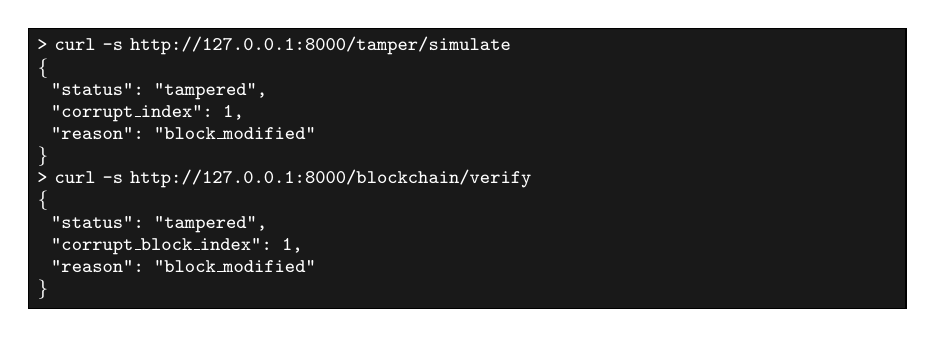
\begin{tikzpicture}
    \node[draw, rectangle, fill=black!90, text=white, text width=0.9\columnwidth, font=\ttfamily\scriptsize] {
      > curl -s http://127.0.0.1:8000/tamper/simulate \\
      \{ \\
      \ \ "status": "tampered", \\
      \ \ "corrupt\_index": 1, \\
      \ \ "reason": "block\_modified" \\
      \} \\
      > curl -s http://127.0.0.1:8000/blockchain/verify \\
      \{ \\
      \ \ "status": "tampered", \\
      \ \ "corrupt\_block\_index": 1, \\
      \ \ "reason": "block\_modified" \\
      \}
    };
  \end{tikzpicture}
  \caption{API response demonstrating immediate detection of a simulated tamper event.}
  \label{fig:tamper_output}
\end{figure}

The `/attestation' endpoint successfully calculated SHA-256 hashes for all model weights and pipeline source files, guaranteeing that the edge deployment had not suffered unauthorized software modifications. 

\subsection{Hardware Tamper Detection}
The simulated hardware tamper monitor (via keyboard interrupt and serial simulation) effectively generated `TAMPER\_DETECTED' events. The integration proved that physical security breaches can be irrevocably logged onto the blockchain, guaranteeing the forensic chain of custody.

\section{Advantages}
\begin{itemize}
    \item \textbf{High Privacy}: Absolute compliance with zero-storage policies through volatile RAM frame handling.
    \item \textbf{Immutable Auditability}: The integration of VPAP and a PoA blockchain ensures forensic-grade logs.
    \item \textbf{Efficient Edge AI}: Dual YOLOv8 optimization allows continuous tracking of PPE, posture, and spatial positioning in real-time.
    \item \textbf{Decentralized Data}: IPFS integration prevents localized data loss and single-point-of-failure vulnerabilities.
\end{itemize}

\section{Limitations}
\begin{itemize}
    \item \textbf{Computational Overhead}: While optimized, dual inference coupled with RSA signing and SHA-256 hashing requires capable edge hardware.
    \item \textbf{IPFS Latency}: The overhead of encrypting and uploading metadata to IPFS can introduce micro-latencies in the event recording pipeline.
\end{itemize}

\section{Future Work}
Future research will investigate optimizing the blockchain consensus mechanism for highly constrained IoT devices (e.g., using lightweight hash functions). Additionally, the system will be extended to support multi-camera spatial tracking, enabling holistic workplace safety monitoring across vast industrial floors. Federated learning will also be explored to continuously improve the YOLOv8 models without centralizing sensitive visual data.

\section{Conclusion}
This paper presented PoseVision, a novel privacy-preserving Edge AI system for workplace safety monitoring. By meticulously combining real-time computer vision (YOLOv8) with cryptographic security constructs (VPAP, PoA Blockchain, IPFS), the architecture proves that stringent industrial safety monitoring does not have to compromise worker privacy. The explicit enforcement of volatile-memory inference alongside immutable, decentralized, and tamper-evident event logging establishes a new benchmark for secure, auditable, and privacy-compliant surveillance systems. The inclusion of a robust hardware monitoring layer further cements the system's viability for deployment in defense and high-security industrial sectors.

\section*{Acknowledgements}
The authors sincerely thank Dr.~K.~N.~Subramanya, Principal of RV College of Engineering (RVCE), Bengaluru, for his encouragement and steadfast institutional support throughout this research. We gratefully acknowledge the Department of Computer Science and Engineering at RVCE for providing the research environment and computational resources that made this work possible.

\begin{thebibliography}{99}

\bibitem{redmon2016you}
J.~Redmon, S.~Divvala, R.~Girshick, and A.~Farhadi,
``You only look once: Unified, real-time object detection,''
\textit{Proceedings of the IEEE conference on computer vision and pattern recognition}, 2016.

\bibitem{bochkovskiy2020yolov4}
A.~Bochkovskiy, C.-Y.~Wang, and H.-Y.~M.~Liao,
``YOLOv4: Optimal Speed and Accuracy of Object Detection,''
\textit{arXiv preprint arXiv:2004.10934}, 2020.

\bibitem{jocher2023yolo}
G.~Jocher, A.~Chaurasia, and J.~Qiu,
``YOLO by Ultralytics,'' 2023. [Online]. Available: https://github.com/ultralytics/ultralytics

\bibitem{chen2019deep}
J.~Chen and X.~Ran,
``Deep learning with edge computing: A review,''
\textit{Proceedings of the IEEE}, vol.~107, no.~8, 2019.

\bibitem{padilla2015privacy}
R.~Padilla et al.,
``Privacy-preserving video surveillance: A review,''
\textit{IEEE Transactions on Information Forensics and Security}, 2015.

\bibitem{mcmahan2017communication}
B.~McMahan et al.,
``Communication-efficient learning of deep networks from decentralized data,''
\textit{Artificial intelligence and statistics}, PMLR, 2017.

\bibitem{zheng2017overview}
Z.~Zheng et al.,
``An overview of blockchain technology: Architecture, consensus, and future trends,''
\textit{IEEE international congress on big data (BigData congress)}, 2017.

\bibitem{christidis2016blockchains}
K.~Christidis and M.~Devetsikiotis,
``Blockchains and smart contracts for the internet of things,''
\textit{IEEE Access}, vol.~4, 2016.

\bibitem{gipp2015decentralized}
B.~Gipp, N.~Meuschke, and A.~Gernandt,
``Decentralized trusted timestamping using the crypto currency bitcoin,''
\textit{iConference 2015 Proceedings}, 2015.

\bibitem{benet2014ipfs}
J.~Benet,
``IPFS-content addressed, versioned, P2P file system,''
\textit{arXiv preprint arXiv:1407.3561}, 2014.

\bibitem{geambasu2009vanish}
R.~Geambasu, T.~Kohno, A.~A.~Levy, and H.~M.~Levy,
``Vanish: Increasing Data Privacy with Self-Destructing Data,''
\textit{USENIX Security Symposium}, 2009.

\bibitem{zhao2024multi}
X.~Zhao, D.~Han, Y.~Bao, J.~Qian, and R.~Yang,
``A Multi-Information Spreading Model for One-Time Retweet Information in Complex Networks,''
\textit{Entropy}, vol.~26, no.~2, 2024.

\bibitem{juliussen2023algorithms}
B.~A.~Juliussen, J.~P.~Rui, and D.~Johansen,
``Algorithms that forget: Machine unlearning and the right to erasure,''
\textit{Computer Law \& Security Review}, 2023.

\bibitem{mohan2025realtime}
D.~S.~S.~Mohan, K.~V.~S.~Chakresh, K.~S.~Reddy, and Y.~Sailaja,
``A Real-Time System for Portfolio Optimization Using Markov Chain Steady-State Analysis,''
\textit{Proc.\ IEEE CSITSS}, 2025, doi: 10.1109/CSITSS67709.2025.11294179.

\bibitem{sailaja2025stochastic}
Y.~Sailaja, S.~Chakote, R.~Shreyashwini, and V.~Khandelwal,
``Stochastic Epidemic Modeling on Networks Using Markov Processes: A Simulation Study,''
\textit{Proc.\ IEEE CSITSS}, 2025, doi: 10.1109/CSITSS67709.2025.11294530.

\end{thebibliography}

\end{document}
